% The finite unit circle x^2+y^2=1 over F_7, with the angle labels k in Z/8.
\documentclass[tikz,border=8pt]{standalone}
\usepackage{amsmath,amssymb}
\begin{document}
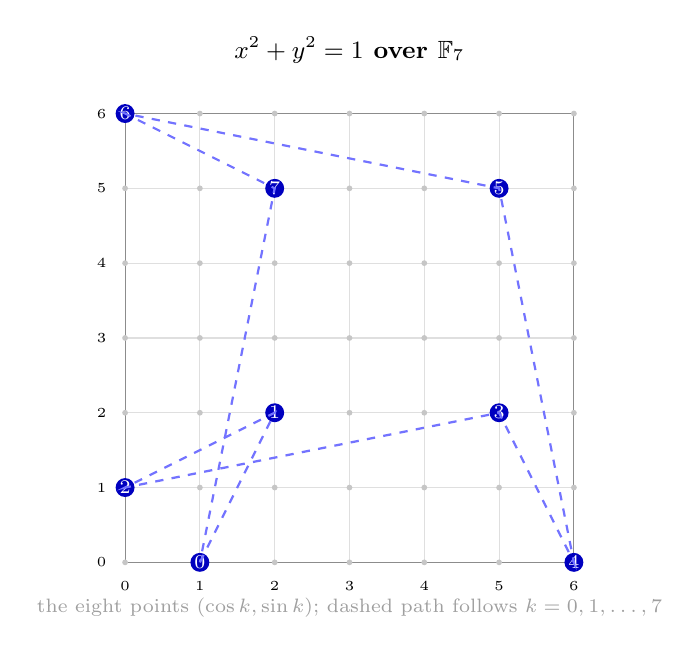
\begin{tikzpicture}[scale=0.95]
  \draw[gray!25] (0,0) grid (6,6);
  \draw[black!45] (0,0) rectangle (6,6);
  \foreach \x in {0,...,6} {%
    \foreach \y in {0,...,6} \fill[gray!45] (\x,\y) circle (1.1pt);}
  \foreach \x in {0,...,6} \node[font=\tiny,below] at (\x,-0.12) {\x};
  \foreach \y in {0,...,6} \node[font=\tiny,left] at (-0.12,\y) {\y};
  % the eight points (cos k, sin k)
  \foreach \x/\y/\k in {1/0/0,2/2/1,0/1/2,5/2/3,6/0/4,5/5/5,0/6/6,2/5/7} {%
    \fill[blue!75!black] (\x,\y) circle (3.6pt);
    \node[font=\scriptsize,text=white] at (\x,\y) {\k};
  }
  % the angle order k = 0,1,...,7
  \draw[blue!55, dashed, line width=0.8pt]
    (1,0)--(2,2)--(0,1)--(5,2)--(6,0)--(5,5)--(0,6)--(2,5)--cycle;
  \node[font=\small\bfseries] at (3,6.85) {$x^2+y^2=1$ over $\mathbb F_7$};
  \node[font=\scriptsize,gray!75] at (3,-0.6)
    {the eight points $(\cos k,\sin k)$; dashed path follows $k=0,1,\dots,7$};
\end{tikzpicture}
\end{document}
